\chapter{Structured interactions as a stabilizing mechanism for competitive communities}\label{chp:1}

% One of the critical unanswered challenges in natural sciences is how ecosystems can produce and sustain the astounding biodiversity we observe in nature. This question has drawn interest from a variety of disciplines, including theoretical ecology, mathematics, and physics.  In this context, modeling the stable coexistence of species competing for limited resources is a particularly challenging task. The presence of dominant intransitive cycles in competitive dynamics is one of the processes that make coexistence mathematically possible. However, intransitive interactions frequently end in neutral cycling of species' relative abundance rather than convergence to a stable equilibrium. Though several processes have been proposed in recent years, there are currently few theories that can adequately explain how different species may coexist in competitive ecosystems. Here, we point out that one of the simplest factors promoting stable species coexistence is the locality in their interactions. We investigate a simplified ecosystem in which members of each species are distributed in a spatial network, where interactions are only feasible between nodes that are physically close to one another. The model allows for extrapolation between local and global competition by varying this distance. Our findings show that species may survive and reach a stable equilibrium if two requirements are satisfied. Namely, individuals need to be embedded in space, and they can only interact with other nearby agents. If one of these components is absent, significant oscillations appear.\\

 %In this chapter, the next section introduces our model, followed by the presentation of the results obtained from numerical simulations in Section~\ref{chp1:2}. Our conclusions are then summarized in Section~\ref{chp1:3}.

Ecosystem stability is a persistent question in ecology \cite{May1972,Chesson2018,Allesina2015}. Given the complexity of ecosystems, it is remarkable the biodiversity that they support over extended periods of time. This has led to extensive interdisciplinary research, with many fields of study, such as statistical physics, computer science, and the physics of disordered systems, applying their tools to ecological problems \cite{Bunin2017Ecological,Sidhom2020Ecological,azaele2016neutral}. Over the years, various mechanisms have been proposed to explain the persistence of biodiversity, including random interaction models \cite{May1972} and niche theory \cite{Chesson2018,Bartomeus2018a}. In particular for competitive communities,  higher-order interactions \cite{Grilli2017Higher-orderModels,Losapio2019,Levine2017BeyondCommunities,battiston2021physics} and intransitivity \cite{may1975nonlinear,Laird2009, kerr2002local,maynard2017diversity,buss1979competitive} have been identified as important factors that contribute to maintaining biodiversity.\\

Mathematical models of competitive communities typically assume that one species will dominate and drive all others to extinction, a phenomenon known as the competitive exclusion principle \cite{hardin1960competitive}. However, we do not find this result in natural systems, and hence numerous mechanisms have been proposed to explain the observed diversity of species.  One such mechanism involves the establishment of dominance relationships among species based on a ``Rock-Paper-Scissors'' tournament, in which species $i$ dominates over $j$, $j$ beats $k$, and $k$ is superior to $i$, forming so-called intransitive cycles. Intransitivity, as we mentioned in Section~\ref{chp:methods:intra}, may play a crucial role in promoting species coexistence \cite{may1975nonlinear,maynard2017diversity}, while relative abundances may be shaped by the structure of dominance relationships among species\cite{Laird2009}. Additionally, intransitive tournaments can be defined probabilistically to increase generality. In that situation, one species does not always out-competes others but it does so with a certain probability, allowing for endogenous stochasticity in the dynamics of these systems.\\

Concerning stability, large oscillations in populations are generally viewed as detrimental to biodiversity because they increase the risk of species extinction due to external perturbations. Mathematical models incorporating intransitive dominance often result in species abundances neutrally cycling around an equilibrium point, which is unlikely to occur in natural systems. To address this issue, researchers have proposed various approaches, including the incorporation of higher-order interactions, which involve the modulation of species interactions by other species \cite{Losapio2019,Levine2017BeyondCommunities}. These interactions can lead to convergence towards equilibrium and help to stabilize the dynamics of the system \cite{Grilli2017Higher-orderModels}. This and other approaches focus mainly on interactions between species and ignore that, within species, individual organisms can compete with multiple partners whose identity can change in space (\textit{i.e.} they ignore structured interactions).\\

However, spatial heterogeneity is another factor that can strongly influence species coexistence \cite{valladares2015species,Dieckmann2000,Lowery2019,Travis2005}. The spatial arrangement of individuals can especially impact the magnitude of their mutual interactions, leading to distinct dynamics. For instance, studies have shown that global oscillations in the rock-scissors-paper game can transition to local oscillations when connections between individuals are rewired while maintaining the same number of interactions for each individual \cite{szolnoki2004phase}. In the same way, the nature of ecological interactions can also influence the spatial distribution of individuals. While various studies have identified space as a driver of species coexistence, it is typically considered to only affect biotic or environmental rates in ecological models \cite{Travis2005,Dieckmann2000}. The spatial patterns that emerge are determined by multiple factors, such as self-organization processes \cite{Pascual2002ClusterEcologies}, spatial disturbances \cite{Lowery2019}, early warning signals of ecological transitions \cite{Kefi2007SpatialEcosystems}, and space-dependent ecological interactions \cite{Dieckmann2000}. These factors contribute to the complex interplay between spatial and ecological dynamics, which can have significant implications for the stability and persistence of ecological systems. \\

 Among the spatially dependent ecological process that can have significant consequences for ecosystem coexistence and diversity, we find seed dispersal \cite{Liao2016,Chave2013}, as well as the growth of sessile organisms like corals \cite{buss1979competitive}. From an empirical perspective, experimental studies with three strains of E. coli have shown that the locality of processes can promote diversity through non-hierarchical competition \cite{kerr2002local}. Similarly, in fungi, competition for space with high levels of intransitivity can foster coexistence among different species \cite{maynard2017diversity}. In coral reefs, intransitive patterns of competition for space can decide the final dominant species \cite{buss1979competitive}. These works suggest that space and intransitivity are crucial ingredients for promoting biodiversity. However, even if their effects have been in the spotlight for years \cite{soliveres2018everything}, the question of the role of space in the emergence and maintenance of stability in competitive intransitive communities, as a way to produce structured interactions, has not been fully explored. \\

In this Chapter, we show that space has a stabilizing effect on competitive communities, similar to the effect caused by higher-order interactions, by examining the competitive dynamics that appear from the spatial proximity between sessile individuals. To begin with, we investigate simplified competitive dynamics where pairs of individuals compete for resources through probabilistic intransitive cycles. We introduce space into this framework explicitly by creating an interaction network between individuals, where nodes represent  individuals of different species and links are drawn according to their distance. The spatial arrangement of individuals limits competition to only adjacent neighbors, reducing their mixing. By varying the minimum distance at which links are created, we can interpolate between local and global interactions to study their impact on the dynamics. For instance, when each individual can interact with every other individual in the system, we recover the classical mean-field case for global competition. This context provides a convenient environment to explore whether the spatial distribution of individuals, in combination with the range of competitive interactions, can function as mechanisms for the maintenance of biodiversity, serving as an alternative to higher-order interactions.\\

\section{\label{chp1:1}Building blocks of a stable competitive community}

We analyze an isolated community made up of a fixed large number of individuals $N$ from various $g$ species, and we consider the impact of space in two different factors: the geographical location of the individuals of the different species and the distance up to which they can interact. The first aspect is represented by a network, where each individual occupies a node representing a physical position. Only one individual can be hosted by a node at a time. These spots may be distributed randomly or regularly spaced. Secondly, regarding interactions,  they compete if there is a link between two individuals. Connections are established according to an interaction range, where long-distance contacts increase global competition and lose spatial correlations. Instead, short ranges result in local interactions between nearby nodes, creating what we call ``structured interactions''. \\

  Under these assumptions, our model is appropriate for organisms that are firmly rooted in one location, so possible target
communities are those mainly governed by local interactions such as shrubs, grasslands, and plants with clonal growth \cite{Dieckmann2000}.
  
\begin{figure}[htbp]
 \centering
 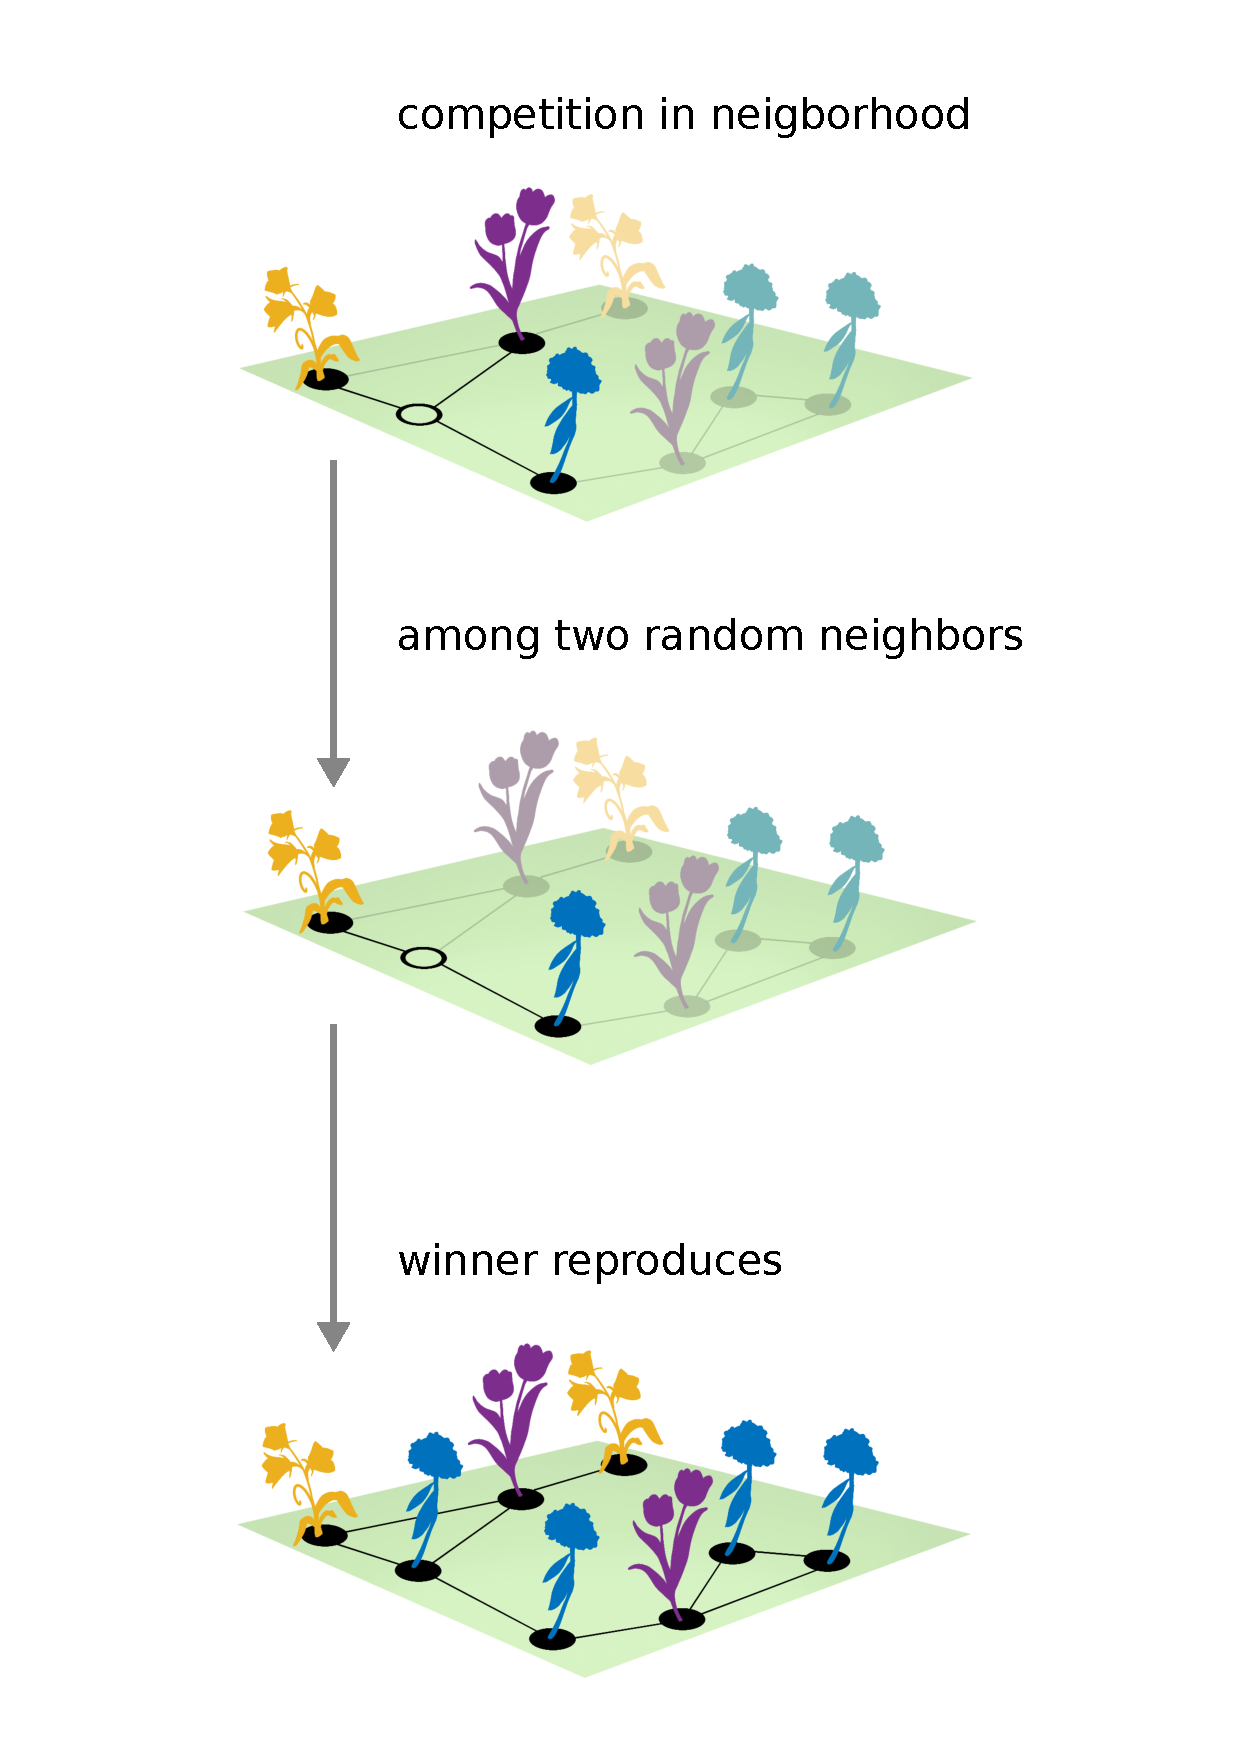
\includegraphics[width =0.8\textwidth]{figures/chp1/fig1.pdf}
 \caption[Competitive dynamics model]{Competitive dynamics are represented schematically in the diagram. We describe the model through the example of plants competing in a forest. With probability $1/N$, a random plant dies, leaving an empty fertile place (an empty node). Of the three neighbors, two of them are chosen at random (highlighted in the center Panel) to compete for placing their seedlings there. The winner is then selected based on the probabilities of the species dominance matrix $H$, and its descendant grows in the empty node. }
 \label{chp1:fig:1}
\end{figure}


\subsection{\label{chp1:1.1}Competitive Dynamics}
 To focus on the relationship between stability and space, we consider a minimal model for competitive communities. Specifically, there are only two ecological processes at play: death (with mortality rates equal for all species) and competition. At each time step, an individual dies, leaving a vacant location that becomes immediately available. This ignites competition among its neighbors to reproduce and fill the location. The neighbors are the individuals within an interaction range that can reach that location. Two of them are randomly selected and compete for placing a descendant. The winner is chosen using a dominance-matrix approach, explained below, and its offspring matures in the next time step (Figure~\ref{chp1:fig:1}). \\

 The $g \times g$ dominance matrix $H$ encodes the winning probability of an individual of species $i$  in competition against an individual of species $j$. The values of $H_{ij}$ for $i> j$ are extracted at random from a uniform distribution [0,1]. We then set  $H_{ji}=1-H_{ij}$, and $H_{ii}  = 0.5$. With these conditions, coexistence is reached when $H$ presents intransitive dominance cycles \cite{Grilli2017Higher-orderModels,Allesina2015PredictingWebs}. Intransitive cycles of competitive dominance occur when $H_{ij} > H_{jk}> H_{ki} > 0.5 $ for some triad $i,j,k$. See Section~\ref{chp:methods:intra} for a short introduction to the importance of intransitivity in ecological systems. \\

To assure the replicability of our results in the numerical simulations, we set $g = 3$ and the following matrix $H$ for our numerical simulations:
 \begin{equation}
 H = 
 \begin{pmatrix}
0.5 & 0.34 & 0.76 \\
0.66 & 0.5 & 0.25 \\
0.24 & 0.75 & 0.5 
\end{pmatrix}. \label{eq:H}
 \end{equation}
Moreover, our conclusions remain valid independently of the number of species and the precise form of matrix $H$ as long as it contains intransitive cycles.

%Moreover, the ecosystem is constrained to have an odd $g$ in the long term in agreement with the equivalent replicator dynamics in \cite{Grilli2017Higher-orderModels}:
%\begin{equation}
%    \frac{d x_i}{ dt} = x_i \sum_{ij} W_{ij} x_j,
%    \label{eq:Pgrilli}
%\end{equation}
%where $W = H-H^t$. The result derives from the fact that Eq.~\ref{eq:Pgrilli} only has an equilibrium $x^*_i \geq 0$ if the dimension of $W$ is odd when $W$ is antisymmetric.  When one species goes extinct, another extinction event must occur to keep the number of species odd.
%



%(from draft_v2)Competitive relationships are hence neither completely  hierarchical nor intransitive and encoding the competitive relationships as the probabilities $H_{ij}$ allows us to range from neutral to complete dominance. The elements $H_{ij}$ are not $\pm 1$ or $0$ as in others intransitivity models \cite{Laird2009}, but take account of a probabilistic intransitivity

\subsection{Interactions' structure}
Once defined the competitive dynamics we model the effect of space. In particular, space is involved in two ways to explore its effect on the dynamics. It is present through the nodes' physical layout and by the distance upon which individuals can compete.
To explore the effect of different spatial arrangements, we employ three different types of networks: a 2D square lattice, an Erd{\H{o}}s-R{\'e}nyi graph, and a Random Geometric Graph (see Section~\ref{chp:methods:networks} for a more detailed description of the networks). \\

%TEXTO INICIAL ANTES DE PASAR PARTE A LOS METODOS: 
%The \textit{2D square lattice} serves as the standard for the most ordered space because of its simplicity and widespread application in ecology \cite{Dieckmann2000,grimm2005IBM,Lowery2019}. Its nodes are discretely and consistently spaced from one another on the unit square. The eight adjacent nodes are thought to be a node's closest neighbors (considering periodic boundary conditions) (left graph of Figure~\ref{chp1:fig:2}a). The 2D lattice, whose nodes are regularly distributed and connected, generates strong spatial correlations.
The \textit{2D square lattice} is our null model of a highly ordered space due to its simplicity and widespread application in ecology \cite{Dieckmann2000,grimm2005IBM,Lowery2019}. It generates strong spatial correlations because nodes are regularly distributed and connected on the unit square (Figure~\ref{chp1:fig:2}a). 

On the other extreme, \textit{Erd{\H{o}}s-R{\'e}nyi graphs} (ER)\cite{erdos1959random} are our baseline for non-spatial interactions. Nodes are randomly connected with probability $p$, regardless of their location (Figure~\ref{chp1:fig:2}c). Consequently, there are no spatial correlations.

Finally, the \textit{Random Geometric Graph} (RGG) \cite{Dall2002RandomGraphs} is a compromise solution in respect of structure and randomness. Nodes are randomly distributed in the unit square and connect if their Euclidean distance is smaller or equal to an interaction radius $R_{RGG}$ (Figure~\ref{chp1:fig:2}b). This point makes an RGG very versatile. Although the network has a disordered structure, it shows strong spatial correlations because of the interaction radius, which allows us to tune continuous distances and investigate the variability in the number of neighbors \cite{cardillo2012,estrada2016,arias2018}.  We have set in this graph, and in the lattice, periodic boundary conditions to avoid irregular properties in the limits of the square. A node very close to the bottom will connect with a node high at the top. \\

Summing up, the ER graph serves as our null model as it lacks spatial structure. The \textit{2D square lattice} represents highly regular interactions, while the RGG strikes a balance between the two models. \\

\begin{figure}[htbp]
 \centering
 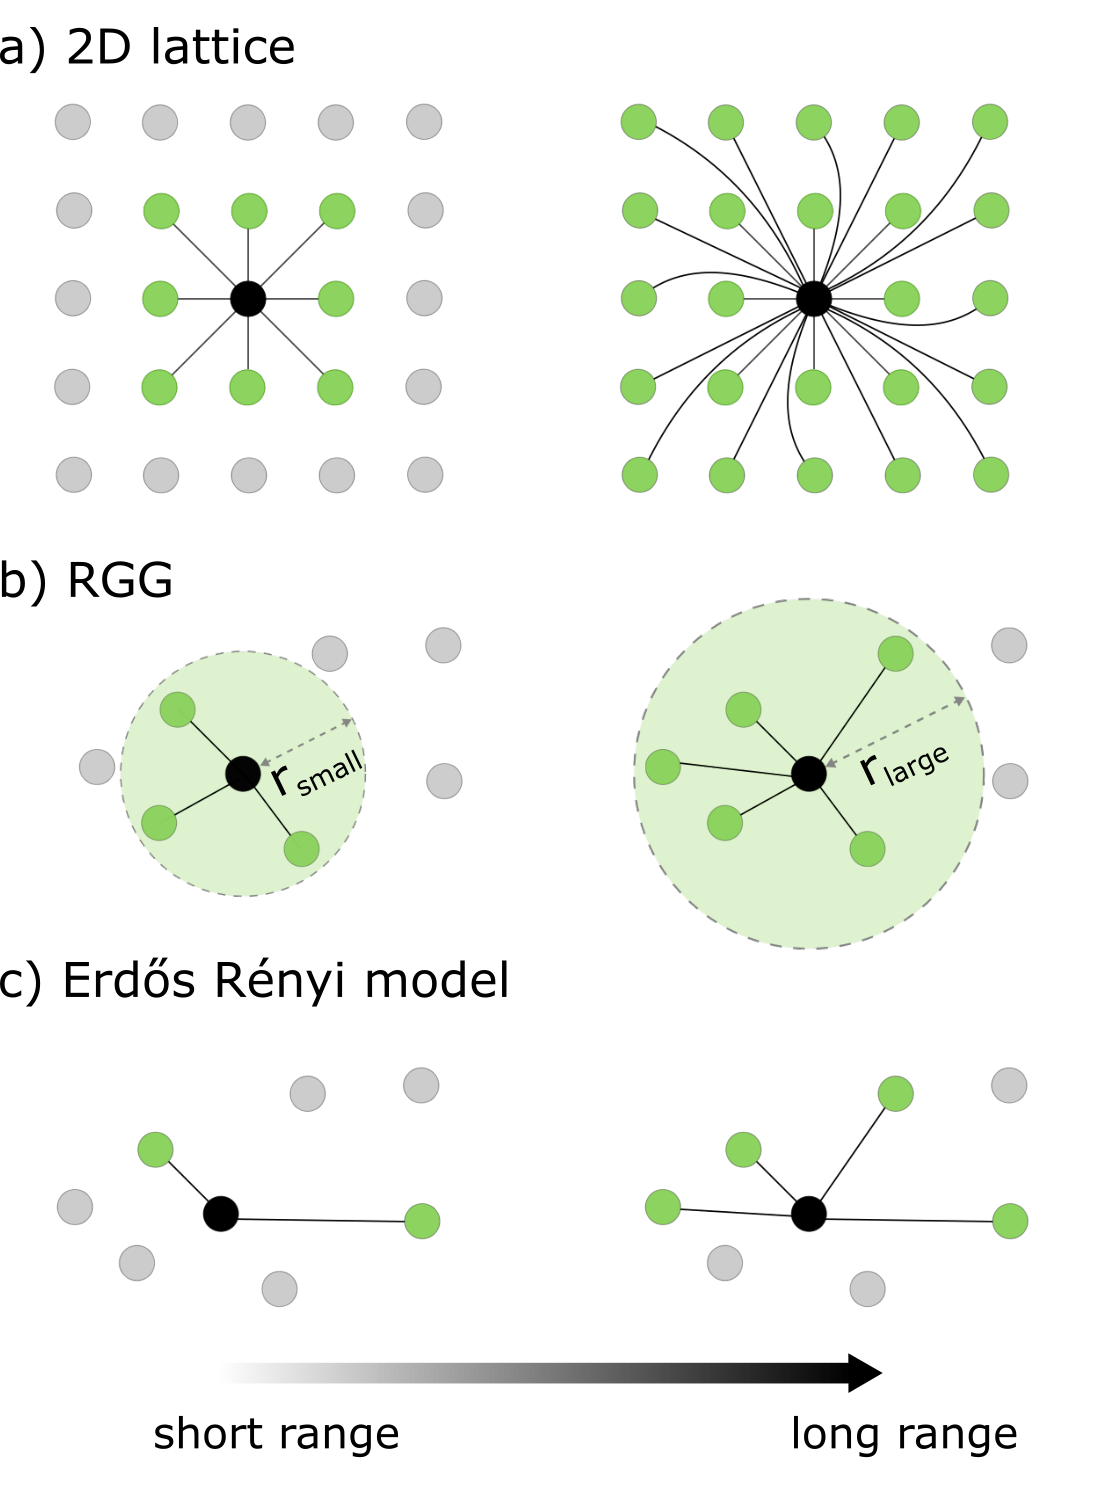
\includegraphics[width =0.75\textwidth]{figures/chp1/fig1.png}
 \caption[Spatial interaction networks]{The three spatial interaction networks under consideration. The black node's neighbors are shown in green for various interaction ranges. (Panel a) The 2D lattice has a homogeneous distribution of nodes. The neighborhood on the left side of the Panel corresponds to the shortest interaction range, and on the right side, we see how it increases when the smallest interaction range has been raised by one unit. (Panel b) For the Random Geometric Graph (RGG), the coordinates of the nodes are set uniformly
 at random in the unit square. Two nodes are linked together if their
 distance is less than $R_{RGG} = r_{small}$ (left side of the Panel)
 or $R_{RGG} = r_{large}$ (right side). (Panel c) The Erd{\H{o}}s-R{\'e}nyi
 graphs do not have any spatial structure because, with probability
 $p$, a pair of nodes is connected regardless of their distance. In Panel c, nodes present the spatial arrangement as in Panel b, but now the neighborhood
 of the black node is randomly determined by linking probabilities
 $p = 0.2$ and $p = 0.4$, respectively.
}
 \label{chp1:fig:2}
\end{figure}
Once defined the structures of our interactions, we now turn to the question of how space is involved in the creation of the links. The interaction range tackles precisely this problem. The range determines who interacts with whom and, ultimately, it defines the individuals that compete for a vacant location that another leaves when it dies. When the interaction range is short, only close nodes compete. More distant nodes join the competition as the range grows, and eventually, the neighborhood size will be large enough to cancel out the influence of nodes' location. Finally, for every network, we trivially get all-to-all competition with the largest interaction range. At that point, we can consider the system to be well-mixed. \\

We regulate the competition from local to global in the different networks by modifying the interaction range. In particular, for square lattices, increasing the interaction range $R_{2D}$ sets connections not only between the nearest nodes but also the second, the third groups of closest neighbors. In the same way, long-range interactions in an RGG are obtained by increasing the interaction radius $R_{RGG}$. In ER networks, node distances do not play any role. Increasing the connection probability $p$ creates larger neighborhoods, but the locations of the neighbors are random. Thus, to compare results across the different network models, it is convenient to quantify the interaction range by the mean degree $\langle k \rangle$. Table~\ref{chp1:tab:1} summarizes the main features of the networks and provides the relationship between the interaction range and $\langle k \rangle$, while the right column of Figure~\ref{chp1:fig:2}a-c gives a glimpse of how the networks look after increasing the interaction range.

\begin{table}[t]
\centering
\caption[Spatial features of network models]{Spatial features (or their absence) of the three considered network models. Further details are explained in Section~\ref{chp:methods}. The average neighborhood size is denoted by $\approx \langle k \rangle$.}
\label{chp1:tab:1}
\begin{tabularx}{\textwidth}{X X c X c}
\hline
\textbf{Network}    &\textbf{Parameter}  &  \textbf{Space}  & \textbf{Connections} & \textbf{$ \langle k \rangle$} \\ \hline \hline
2D lattice & interaction radius, $R_{2D}$  &   ordered     & Chebyshev distance  & $\sum_{r = 1}^{R_{2D}} 8 r$              \\ \hline
RGG        &  interaction radius, $R_{RGG}$  & random    & Euclidean distance  & $\pi R_{RGG}^2(N-1)$                \\ \hline
ER         &    connection probability, $p$   & random & random              & $\approx p(N-1)$  \\
\hline
\end{tabularx}
\end{table}

\section{\label{chp1:2}Results}
%%%%%%%%%%%%%%%%%%%%%%%%%%%% RESULTS
Once the model has been defined, we begin an extensive analysis of it using Monte Carlo simulations. At the start of each simulation, species inside each node are initially assigned at random with  uniform probability $1/g$. The variable $n_{i,\nu}$ will take the value of 1 if species $i$ is present at node $\nu$, and $0$ otherwise. Since a node can only host one individual at a time, then $\sum_i^g n_{i,\nu}=1$, $\forall \nu$. We use an asynchronous update (each time step, just one node is selected to die) and define a generation as $N$ updates. To ensure that on average every node has experienced death events, we simulate during at least $N$ generations. Lastly, we monitor the relative abundance of individuals of each species in the system $x_i(t) \equiv N^{-1}\sum_\nu^N n_{i,\nu}$. \\

To help understand the  macroscopic state of the system, we employ the relative abundances $x_i$. In fact, since for every $t$, we have $\sum_{i}^{g} x_i(t) = 1$, this expression means that the relative abundances represent a point in the $(g-1)$-simplex (the portion of the $\sum_{i=1}^{g} x_i=1$ plane which $x_i \geq 0, \, \forall i$). The vertices of the simplex, in particular, correspond to a population of just one species. As time evolves, the variation in relative abundances follows a trajectory confined in the simplex. These trajectories characterize the state of the system and therefore the simplex may be seen as a representation of the phase space. \\

\begin{figure*}[t!]
     \centering
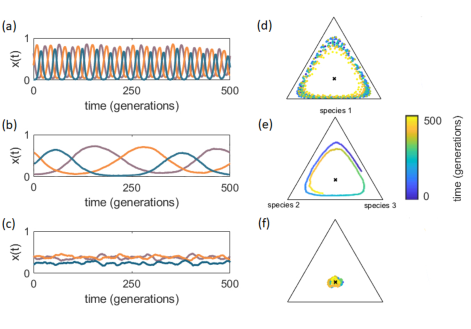
\includegraphics[width=1.1\textwidth]{figures/chp1/fig3.pdf}
 \caption[Temporal evolution of relative abundances and simplex representation]{(Panels a,b,c) Temporal evolution of relative abundances $x(t)$ for the different interaction scenarios in a RGG with $ N = 10^4$. (Panel a) All-to-all interactions: individuals compete for any empty node as the radius covers the whole plane ($R_{RRG} = R_{max} = \sqrt{2}$). (Panel b) Long-range interactions: the radius is reduced to $R_{RGG} = 0.15$, which corresponds to an average degree $\langle k \rangle \simeq 706$. These two radii create a similar scheme in that the community lacks structure and leads to wide oscillations. (Panel c) Short-range interactions: now $R_{RGG} = 0.03$ and $\langle k \rangle \simeq 28$. In this situation, the system is spatially structured and abundances do not heavily fluctuate. (Panels d,e,f) The trajectories of the left Panels are represented on the 2-simplex (the region of the $x_1 + x_2+ x_3 = 1$ plane in which $x_1,x_2,x_3 \geq 0$). The view of the plots is set perpendicular to the simplex plane. Abundances oscillate in wide cycles around what seems an equilibrium point (black cross) for all-to-all (Panel d) and long-range interactions (Panel e). When interactions are short-range (Panel f), abundances are restricted to an area close to the equilibrium. For all Panels, the trajectories are displayed once the transient has vanished.}
\label{chp1:fig:3}
\end{figure*}
\subsection{\label{chp1:2.1}Temporal evolution}

To begin our analysis, we look at the temporal evolution of species abundances for the most straightforward scenario of three competing species, $g=3$. Unless otherwise noted, we always employ the same dominance matrix, given in Eq.~\eqref{eq:H}, which produces results that are typical of any other randomly generated $H$ with competitive intransitive cycles. We find that the behavior through time varies depending on the spatial distribution of species (the networks) and the proximity of their interactions (the interaction range). \\

Cycles of wide amplitude in species abundances occur in communities with no spatial structure, as ER graphs or for all-to-all interactions (Figure~\ref{chp1:fig:3}a). Large fluctuations can also be seen in structured communities (RGG and 2D lattice) with long-range interactions. This behavior is consistent with the mean-field approximation's prediction of the dynamics (see Appendix~\ref{appen:MF}). However, the amplitude of the oscillations is unaffected by the initial conditions, suggesting that they are limit-cycle oscillations, which are qualitatively distinct from the neutral oscillations anticipated by the mean-field theory. \\

Differently, in the two spatial networks considered, decreasing the interaction range reduces the amplitude of the oscillations. For a sufficiently short range,  abundances only slightly fluctuate in the vicinity of an equilibrium state, as it can be seen in Figure~\ref{chp1:fig:3}c.  \\

The value of that state is, for all analyzed cases, the equilibrium fixed point obtained from the mean-field approximation (which is $(x_1,x_2,x_3)=(0.374, 0.383, 0.243)$ for the matrix $H$ in Eq.~(\ref{eq:H})). Returning to the oscillatory case, we also recover the same values if we calculate the temporal average of the relative abundances for the same matrix $H$.  \\

These findings call for further analysis since they show a non-trivial dependence of the dynamics with the interaction range. In the next Subsections, we systematically examine the impact of the interaction range and network structure on the dynamics of the species.

\subsection{\label{chp1:2.2}Dynamical behavior depends on structured interactions} 

As a first step towards getting a better understanding of the dynamics, we define a measure to characterize the system's behavior for each interaction range and structure. In this case, the magnitude of the oscillations is not a reliable indicator because of the stochastic simulations' noisy dynamics. Thus, we focus on the mean area encompassed by the system's trajectory on the simplex, which is measured according to Appendix~\ref{appen:AreaSimplex}. The intuition for this choice is that a trajectory takes up a limited area when the system fluctuates with small amplitude around some equilibrium abundances,  (Figure~\ref{chp1:fig:3}f), whereas larger oscillations cover much broader areas (Figure~\ref{chp1:fig:3}d,e).  \\

After we've established our metric for describing the dynamics, we can study the impact of space. To do so, we keep $H$ fixed across all simulations while changing the interaction range for each type of graph. This procedure allows us to alter the underlying network structures, and go from highly-structured communities to systems for which the effect of space is diluted due to the large interaction range. The ER graphs, however, pose a problem since we are unable to define distances across them. For those graphs, we utilize the degree as a substitute for the interaction range. This substitution is feasible because the interaction range determines both the distance up to nodes compete and their degree. In that way, we can now compare the results for the ER graphs with the two spatial networks.  \\

\begin{figure}[t!]
    \centering
    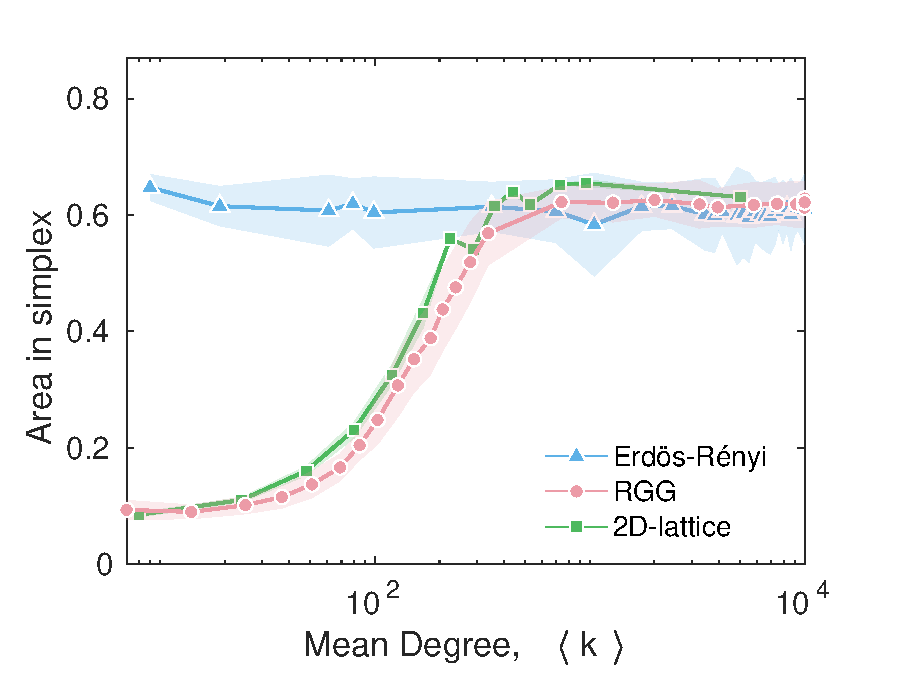
\includegraphics[width=0.8\textwidth]{figures/chp1/fig4.pdf}
    \caption[Impact of average degree on the area in simplex]{Average area inside the trajectory over the 2-simplex of a 3-species community as a  function of average degree $\langle k \rangle$ for the different networks of $N = 10^4$ nodes. The dominance matrix $H$ of Eq.~(\ref{eq:H}) is used for all networks. Each point represents the mean area over $50$ simulations, each starting with different initial conditions and network structures. The areas have been calculated excluding the $5\%$ of out-layer points of the trajectories. Shades indicate the $95\%$ confidence interval. The procedure to compute the areas from time series is explained in Appendix~\ref{appen:AreaSimplex}.}
    \label{chp1:fig:4}
\end{figure}

We start by simulating the ER graphs, i.e. the situation where the system has no spatial structure (blue marks in Figure~\ref{chp1:fig:4}). We increase the average degree to focus solely on the effect of the interaction network, leaving aside any spatial constraints. The simulations present large oscillations for all values of the degree. These wide fluctuations translate into high area coverage for all interaction ranges and, therefore, we can conclude that the size of the neighborhood does not affect the dynamics. \\

However, this picture changes totally when we consider spatially structured interactions. In both the RGG and 2D lattice, the systems show different behavior for short interaction ranges, that correspond to having a low mean degree. In that regime, the dynamics stabilizes around the equilibrium (the cross in Figure~\ref{chp1:fig:3}), covering a tiny area in the phase space (pink and green points in Figure~\ref{chp1:fig:4}). However, as we increase the interaction range and hence increase $\langle k \rangle$, the results of the ER networks are recovered, and we observe large oscillations again. For both networks, the transition between these two regimes occurs when the average degree is $ 50 \lesssim \langle k \rangle \lesssim 100$ for a network of $N = 10^4$ nodes.
 
As a result of these findings, the following intuitive picture emerges: when we consider long-range interactions --e.g. large mean degrees--  we obtain large oscillations, regardless of whether the networks have spatial structure or not. The period and  amplitude of these oscillations are independent of the initial conditions, which suggests they are of the limit-cycle type. In the limit of long-range interactions, the mean-field approximation is expected to be valid, and indeed it correctly predicts the oscillatory behavior (see Appendix~\ref{appen:MF}). But this approximation fails to give the limit-cycle behavior as it predicts instead neutral oscillations. On the other hand, when we constrain competition to short-range interactions, the dynamics stabilize around some fixed point $x^*$ if and only if the networks have some spatial structure by construction, i.e. for the RGG and 2D lattice. \\

Lastly, to test the robustness of our results we also investigated the influence of the model's parameters. Varying the number of individuals $N$ does not strongly modifies the shape of the curve, just it becomes more gradual for larger $N$. The results are still qualitatively the same. We also found results that were nearly identical when $g = 5$ (not shown), except for a higher probability of extinction due to long-range interactions.

\subsection{\label{chp1:2.3}Spatial configurations}

So far, only the behavior  of the species relative abundances $x_i$ has been explored, showing a dependency on the spatial fabric of the networks the species are competing in. To understand this behavior, we turn to directly observe the spatial organization of the species. In Figure~\ref{chp1:fig:5}, we show two different snapshots of a 3-species community in a 2D square lattice. The two images only differ in the interaction range. \\

%To better understand the mechanism behind the reported behavior, we show in Figure~\ref{chp1:fig:5}.

With short ranges (Figure~\ref{chp1:fig:5}a), species form mono-specific patches. Inside the patches, death events  do not contribute to variations in relative abundance because competition is among individuals of the same species. And hence, changes in $x_i$ can only happen along the patches' borders, where different species are in contact. This characteristic makes patches more robust to invasion from other species. In turn, it decelerates the dynamics and reduces the possibility of large oscillations.  \\

\begin{figure*}[t!]
 \centering
  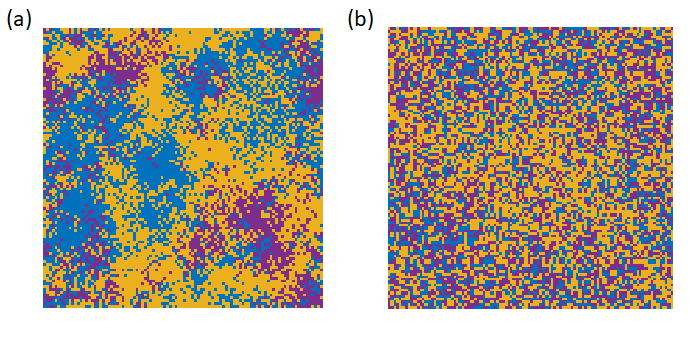
\includegraphics[width=1.0\linewidth]{figures/chp1/fig5.png}
\caption[Spatial organization for different interaction radius]{Spatial organization of a 3-species community in a 2D lattice of $N=10^4$ and dominance matrix $H$ of Eq.~(\ref{eq:H}). Each species is depicted with a different color, matching Figure~\ref{chp1:fig:3}a-c. (Panel a) Short-range interactions: only the $8$ closest neighbors at distance $R_{2D} = 1$ compete for the vacant node left by an individual when dies (see the left graph at Figure~\ref{chp1:fig:2}a). (Panel b) Long-range interactions: $360$ neighbors ($R_{2D} = 9$) participate now in the competition. Videos for the two ranges of interactions are publicly available in \cite{videos}.} \label{chp1:fig:5}
\end{figure*}

With long-range interactions (Figure~\ref{chp1:fig:5}b), vacant nodes can be reached by many individuals from different species, blocking the formation of single-species clusters. The lack of patches would avoid reaching a steady state, generating large-scale oscillations: the homogeneous solution predicted by mean-field theory. Videos of the temporal evolution in the two regimes are available \cite{videos}. \\

The latter results of Figure~\ref{chp1:fig:5} imply that short-range interactions decrease the system's effective competition by lowering the probability of interactions between individuals of different species. To confirm this hypothesis, we compute $\langle P_{ij} \rangle$, the average probability that species $i$ and $j$ compete for a vacant node when interactions are short. This probability is calculated numerically by keeping track of how many times species $i$ and $j$ have been chosen to compete, and then averaging across the simulation's duration. We then compare it with the expected value for the all-to-all case $\overline{P}_{ij}$ that simply is the product of the relative abundances of species $i$ and $j$ at the mean-field equilibrium, i.e. $\overline{P}_{ij}=x_i^* x_j^*$.  \\

In our example system from Eq.~(\ref{eq:H}), we have

$x^*=(0.374, 0.383, 0.243)$, thus:
 \begin{equation}
\overline{P}_{ij} =
\begin{pmatrix}
0.1399 & 0.1432 & 0.0909\\
0.1432 & 0.1467 & 0.0931\\
0.0909 & 0.0931 & 0.0590
\end{pmatrix} 
\label{eq:mata2a}
\end{equation}
And the obtained matrix $\langle P_{ij} \rangle$ in a RGG with short-range interactions ($N = 10^4$, $R_{RGG} = 0.022$ and $\langle k \rangle \simeq 15$) is:
\begin{equation}
\langle P_{ij} \rangle =
\begin{pmatrix}
\textbf{ 0.2160} & 0.0965 & 0.0597\\
 0.0965 & \textbf{0.2241} & 0.0659\\
 0.0597 & 0.0659  & \textbf{ 0.1156}
\end{pmatrix} \ ,
\label{eq:matshort}
\end{equation}
where same-species competition $\langle P_{ii} \rangle$ has been highlighted in boldface. \\

We observe that intra-species competition $\langle P_{ii} \rangle$  has a significantly higher probability to occur than the inter-species competition (the off-diagonal terms $\langle P_{ij} \rangle$) for short-range interactions than in the all-to-all case. This shows that the patches, created exclusively in structured communities with short-range interactions, reduce the effective inter-specific competition.  \\

\begin{figure}[t!]
 \centering
 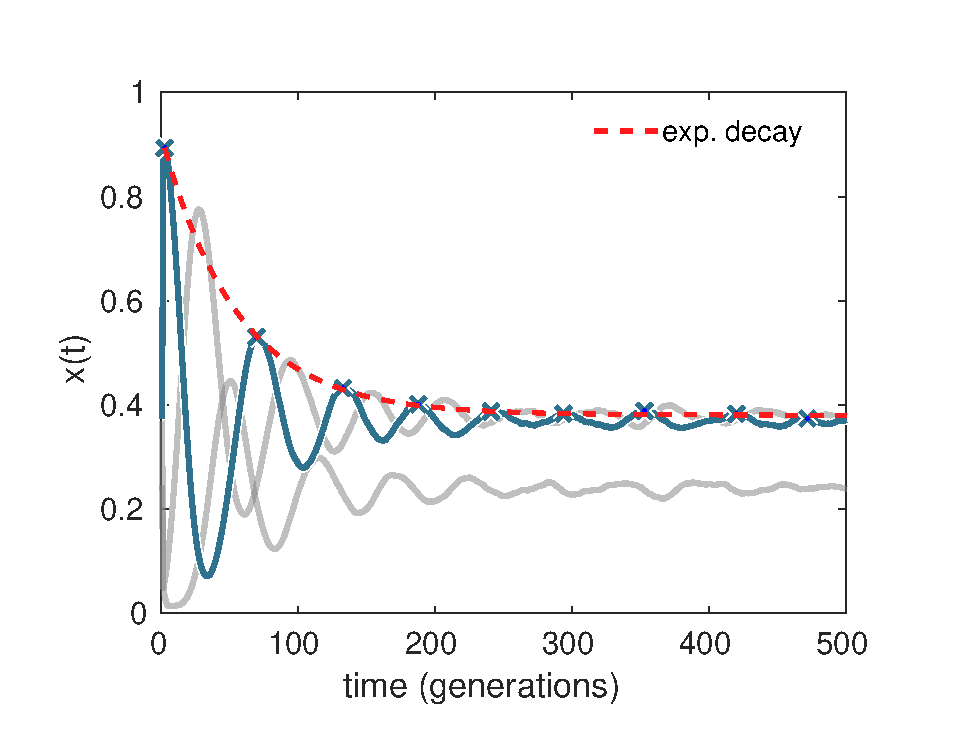
\includegraphics[width=0.8\textwidth]{figures/chp1/fig6.pdf}
  \caption[Time evolution of the recovery from a pulse perturbation]{Recovery from a $90 \%$ pulse perturbation in a 3-species system with $H$ from Eq.~(\ref{eq:H}). The relative abundance of the blue species is artificially boosted from its equilibrium value to be the $90 \%$ of the entire population, while the  other species' relative abundances (in gray) are proportionally reduced. The system is embedded in an RGG of $10^4$ nodes and $R_{RGG} = 0.03$. The red curve is the fit of the local maxima of the relative abundance (blue crosses) to the exponential function, resulting in $a e^{-\alpha} + b$ with $\alpha = 0.018$, $a = 0.53$ and $b = 0.38$.}
    \label{chp1:fig:6}
\end{figure}

\subsection{\label{chp1:2.4}Stability and fluctuations}

Once understood the mechanism responsible for the stabilization of the dynamics in the short-range regime, we turn to check
the stability of that regime. To do so, we investigate how the system reacts to pulse perturbations of various intensities. In the simulations, this is done by imposing an abrupt change in one species' abundance and recording the time required to return to the original state. More precisely, the abundance of a random species is suddenly increased to cover a large portion of the system, while the other species' abundances are proportionately decreased. In Figure~\ref{chp1:fig:6}, we show the evolution 
after a $90 \%$ perturbation of one species'  abundance in an RGG with $R_{RGG}=0.03$ (short range). The system returns to equilibrium while the disturbance decays exponentially. So Figure~\ref{chp1:fig:6} demonstrates that the dynamics can bounce back even with such a large perturbation. \\

\begin{figure}[t!]
 \centering
 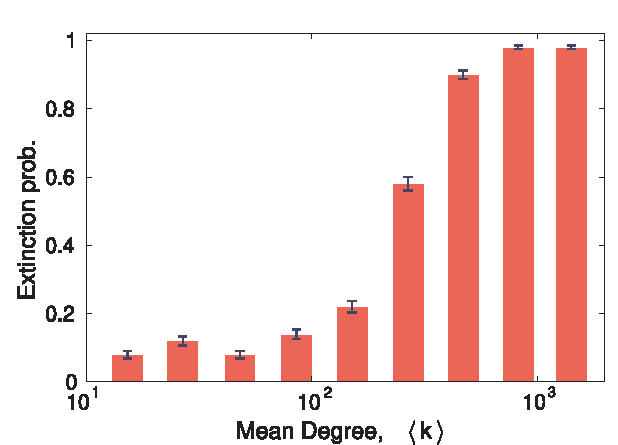
\includegraphics[width=0.8\textwidth]{figures/chp1/fig7.pdf}
  \caption[Extinction probability as a function of the average degree]{ Extinction probability as a function of the average degree. We have varied the interaction radius from short to long ranges. The communities are in an RGG of $N=10^4$ individuals governed by $H$ from Eq.~\eqref{eq:H}. Each red bar corresponds to the mean over $50$ different networks --different simulations-- and the error bars are the $95\%$ confidence intervals.}
    \label{chp1:fig:7}
\end{figure}

However, perturbations could also lead to extinctions since we are simulating a finite system. In such a scenario, the latter fixed point for the macroscopic variables $x_i$ would be lost. To examine when this case occurs, we systematically measure the probability of extinction of one species after a pulse perturbation as a function of the mean degree. In particular, we define the probability of extinction of one species as the fraction of simulations in which at least one species gets extinct following a perturbation. Starting with a $N=10^4$ community in an RGG, we measure those probabilities for increasing interaction radius after a $90\%$ perturbation. Consistently with the previous results, Figure~\ref{chp1:fig:7} shows that the probability falls to less than $10\%$ for small degrees, but extinctions are almost certain for larger neighborhoods, making the long-range interaction regime not robust. \\

\begin{figure}[t!]
 \centering
 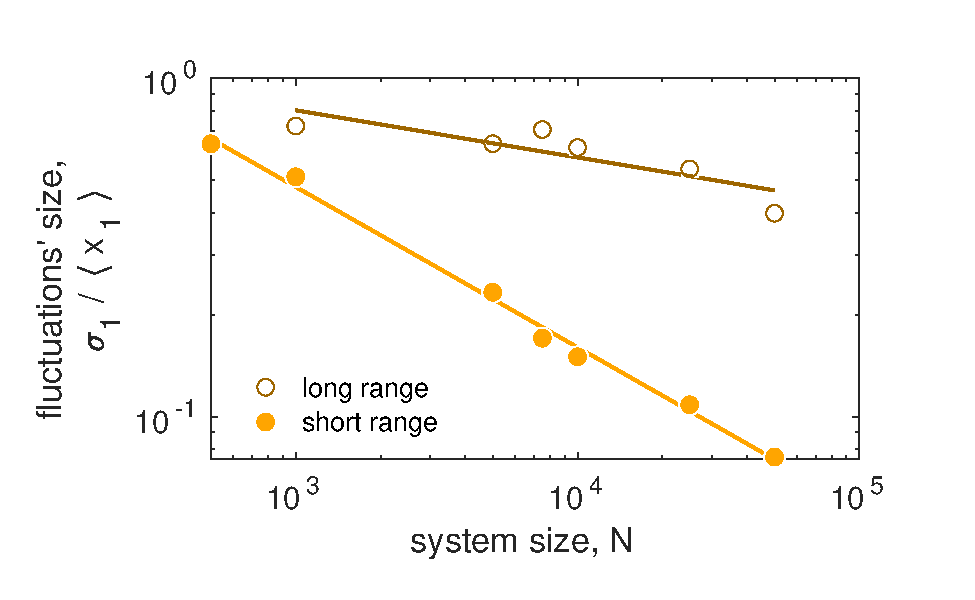
\includegraphics[width=0.8\textwidth]{figures/chp1/fig8.pdf}
  \caption[Interplay between fluctuations' scaling and system size]{Fluctuations' scaling as a function of the system size $N$. We choose the coefficient of variation of species 1 ($\sigma_1/\mean{x_1}$) to be a proxy for fluctuations. Each point is the average over $10$  simulations where the variance $\sigma_1$ and mean relative abundance $\mean{x_1}$ have been calculated over at least $\Delta t = 10^8$ time-steps after the transient. Communities with short-range interactions have an average degree $\langle k \rangle = 15 \pm 2$, and decrease their fluctuations with the size of the system as $\sigma_1/\mean{x_1}\sim N^{-0.47}$, consistent with a scenario with no correlations. For the settings with long-range interactions ($\langle k \rangle = 980 \pm 190$), the scaling of the relative fluctuations goes as $N^{-0.14}$. The simulations have been performed over RGG, with $g =3$ and $H$ of Eq.~(\ref{eq:H}), as usual.}
    \label{chp1:fig:8}
\end{figure}

Finally, we conclude our analysis by studying the nature of the fluctuations around the equilibrium for both short and long-range interactions. To do so, we measure how the size of the fluctuations scales with the system's size. The size is defined as the coefficient of variation of the relative abundance of each species $i$: $\sigma_i/\langle x_i \rangle$. Figure~\ref{chp1:fig:8} shows the scaling for one species in RGG of different sizes and interaction ranges. For short-range interactions, which produce small degrees ($\langle k \rangle = 15 \pm 2$), we observe a scaling exponent of $0.47$. The value is pretty close to $0.5$, the one expected for residual fluctuations that arise from the stochastic noise due to the finite size of the system. As a result, the possibility that the observed fluctuations were truly oscillatory behavior of small amplitude is ruled out. In turn, for networks with larger degrees ($\langle k \rangle = 980 \pm 190$), we find an exponent of $0.14$. In this situation, fluctuations represent an actual ecological signal that results from the interactions in an environment with high mixing. \\

\section{Discussion}
 \label{chp1:3}

Many attempts have been made to provide a biological basis for the robustness of biodiversity in natural ecosystems, especially for those communities governed by competition. Here, we have demonstrated that spatial interactions alone lead to the stability of multispecies communities by a minimum model of intransitive competition. \\
 
We have analyzed  a model where individuals compete in a structured environment with intransitive dominance cycles. We have compared different spatial configurations, from regular lattices to random connections that outweigh the effect of space. Our results reveal that spatial interactions confined to nearest neighbors promote the stable coexistence of different species, while long-range interactions cause species' relative abundances to fluctuate endlessly. \\

 By focusing on the spatial organization of the individuals, we found that local interactions enable species to survive by forming mono-specific patches, that decrease the effective competition experienced by each individual because it only happens at their borders. This clustered configuration slows down the dynamics, dramatically damping out fluctuations and leading to stability. Per contra, mean-field approximations of the dynamics do not match the latter results. This is, however, not unexpected given how much the dynamics depend on the spatial correlations that the short-range interactions produce. \\




